\documentclass[fontsize=12pt, paper=a4, headinclude, twoside=false, parskip=half+, pagesize=auto, numbers=noenddot, open=right, toc=listof, toc=bibliography, hidelinks]{scrreprt}
% PDF-Kompression
\pdfminorversion=5
\pdfobjcompresslevel=1
% Allgemeines
\usepackage[automark]{scrpage2} % Kopf- und Fußzeilen
\usepackage{amsmath,marvosym} % Mathesachen
\usepackage[T1]{fontenc} % Ligaturen, richtige Umlaute im PDF
\usepackage[utf8]{inputenc}% UTF8-Kodierung für Umlaute usw
\usepackage{booktabs} % Tabellen
\usepackage{tablefootnote}
% Schriften
\usepackage{mathpazo} % Palatino für Mathemodus
%\usepackage{mathpazo,tgpagella} % auch sehr schöne Schriften
\usepackage{setspace} % Zeilenabstand
\onehalfspacing % 1,5 Zeilen
% Schriften-Größen
\setkomafont{chapter}{\Huge\rmfamily} % Überschrift der Ebene
\setkomafont{section}{\Large\rmfamily}
\setkomafont{subsection}{\large\rmfamily}
\setkomafont{subsubsection}{\large\rmfamily}
\setkomafont{chapterentry}{\large\rmfamily} % Überschrift der Ebene in Inhaltsverzeichnis
\setkomafont{descriptionlabel}{\bfseries\rmfamily} % für description-Umgebungen
\setkomafont{captionlabel}{\small\bfseries}
\setkomafont{caption}{\small}
% Sprache: Deutsch
\usepackage[ngerman]{babel} % Silbentrennung
% PDF
\usepackage[ngerman,pdfauthor={Georg Donner},  pdfauthor={Georg Donner}, pdftitle={Themenspezifische Gruppierung deutscher Online-Zeitungen mit Natural Language Processing}, breaklinks=false,baseurl={}]{hyperref}
\usepackage[final]{microtype} % mikrotypographische Optimierungen
\usepackage{url} % ermögliche Links (URLs)
\usepackage{pdflscape} % einzelne Seiten drehen können
% Tabellen
\usepackage{multirow} % Tabellen-Zellen über mehrere Zeilen
\usepackage{multicol} % mehrere Spalten auf eine Seite
\usepackage{tabularx} % für Tabellen mit vorgegeben Größen
\usepackage{longtable} % Tabellen über mehrere Seiten
\usepackage{array}
%  Bibliographie
\usepackage{bibgerm} % Umlaute in BibTeX
% Bilder
\usepackage{graphicx} % Bilder
\usepackage{color} % Farben
\graphicspath{{images/}} % Lege den Standardpfad mit Bilder fest
\DeclareGraphicsExtensions{.pdf,.png,.jpg} % bevorzuge pdf-Dateien vor den anderen
\usepackage{subcaption}  % mehrere Abbildungen nebeneinander/übereinander
\usepackage[all]{hypcap} % Beim Klicken auf Links zum Bild und nicht zu Caption gehen
% Bildunterschrift
\setcapindent{0em} % kein Einrücken der Caption von Figures und Tabellen
\setcapwidth{0.9\textwidth} % Breite der Caption nur 90% der Textbreite, damit sie sich vom restlichen Text abhebt
\setlength{\abovecaptionskip}{0.2cm} % Abstand der zwischen Bild- und Bildunterschrift
% Quellcode
% für Formatierung in Quelltexten, hier im Anhang
\usepackage{listings}
\definecolor{grau}{gray}{0.25}
\lstset{
	extendedchars=true,
	basicstyle=\tiny\ttfamily,
	%basicstyle=\footnotesize\ttfamily,
	tabsize=2,
	keywordstyle=\textbf,
	commentstyle=\color{grau},
	stringstyle=\textit,
	numbers=left,
	numberstyle=\tiny,
	% für schönen Zeilenumbruch
	breakautoindent  = true,
	breakindent      = 2em,
	breaklines       = true,
	postbreak        = ,
	prebreak         = \raisebox{-.8ex}[0ex][0ex]{\Righttorque},
}
% linksbündige Fußboten
\deffootnote{1.5em}{1em}{\makebox[1.5em][l]{\thefootnotemark}}

\typearea{14} % typearea berechnet einen sinnvollen Satzspiegel (das heißt die Seitenränder usw.) siehe auch http://www.ctan.org/pkg/typearea. Diese Berechnung befindet sich am Schluss, damit die Einstellungen von oben berücksichtigt werden

\usepackage{scrhack} % Vermeidung einer Warnung


% Eigene Befehle %%%%%%%%%%%%%%%%%%%%%%%%%%%%%%%%%%%%%%%%%%%%%%%%%5
% Matrix
\newcommand{\mat}[1]{
      {\textbf{#1}}
}
\newcommand{\todo}[1]{
      {\colorbox{red}{ TODO: #1 }}
}
\newcommand{\todotext}[1]{
      {\color{red} TODO: #1} \normalfont
}
\newcommand{\info}[1]{
      {\colorbox{blue}{ (INFO: #1)}}
}
% Hinweis auf Programme in Datei
\newcommand{\datei}[1]{
      {\ttfamily{#1}}
}
\newcommand{\code}[1]{
      {\ttfamily{#1}}
}
% bild mit defnierter Breite einfügen
\newcommand{\bild}[4]{
  \begin{figure}[!hbt]
    \centering
      \vspace{1ex}
      \includegraphics[width=#2]{images/#1}
      \caption[#4]{\label{img.#1} #3}
    \vspace{1ex}
  \end{figure}
}
% bild mit eigener Breite
\newcommand{\bilda}[3]{
  \begin{figure}[!hbt]
    \centering
      \vspace{1ex}
      \includegraphics{images/#1}
      \caption[#3]{\label{img.#1} #2}
      \vspace{1ex}
  \end{figure}
}

% Bild todo
\newcommand{\bildt}[2]{
  \begin{figure}[!hbt]
    \begin{center}
      \vspace{2ex}
	      \includegraphics[width=6cm]{images/todobild}
      %\caption{\label{#1} \color{red}{ TODO: #2}}
      \caption{\label{#1} \todotext{#2}}
      %{\caption{\label{#1} {\todo{#2}}}}
      \vspace{2ex}
    \end{center}
  \end{figure}
}
 % Importiere die Einstellungen aus der Präambel
% hier beginnt der eigentliche Inhalt
\begin{document}
\pagenumbering{Roman} % Seitenummerierung mit großen römischen Zahlen 
\pagestyle{empty} % keine Kopf- oder Fußzeilen auf den ersten Seiten

% Titelseite
\clearscrheadings\clearscrplain
\begin{center}
\begin{Huge}
Themenspezifische Gruppierung deutscher Online-Zeitungen mit Natural Language Processing\\
\end{Huge}

\vspace{8mm}
Bachelorarbeit\\
\vspace{0.4cm}
\vspace{2 cm}
Georg Donner\\
Matrikel-Nummer 553821\\
\vspace{8cm}
\begin{tabular}{rl}
{\bfseries Betreuer} & Prof. Dr. Gefei Zhang\\
{\bfseries Erstprüfer} & Prof. Dr. Gefei Zhang\\
{\bfseries Zweitprüfer} & Prof. Dr. Barne Kleinen\\
\end{tabular}

\end{center}
\clearpage

\pagestyle{useheadings} % normale Kopf- und Fußzeilen für den Rest

\tableofcontents % erstelle hier das Inhaltsverzeichnis
\listoffigures % erstelle hier das Abbildungsverzeichnis
\listoftables % Tabellenverzeichnis
\clearpage

% richtiger Inhalt
\pagenumbering{arabic} % ab jetzt die normale arabische Nummerierung
\chapter{Einleitung}
Natural Language Processing ist ein großes Feld, welches besonders in der letzten Zeit im Zuge der Digitalisierung viel an Aufmerksamkeit und Wichtigkeit gewonnen hat. Es ermöglicht uns Informationen schneller zu finden, Systeme durch gesprochene Sprache zu steuern oder ganze Texte zu generieren. Eine weitere Aufgabe ist es, eine große Menge an Texten in Kategorien einzuteilen, um die Daten auf eine gewünschte Teilmenge für eine spezifischere Suche oder Analyse zu reduzieren. Die Kategorisierung der Dokumente nach ihrem Inhalt ist hier der häufigste Anwendungsfall, es ist aber auch möglich Texte nach ihrem generellen Genre oder Schreibstil zu vergleichen.

Diese Arbeit wird am Beispiel deutscher Online-Zeitungen untersuchen, welche Möglichkeiten es gibt Texte unabhängig von ihrem Inhalt zu vergleichen. Dabei werden lexikalische, morphologische und syntaktische Merkmale, aber auch die Verwendung inhaltlich irrelevanter Wörter als Features verwendet. Es wird überprüft, inwiefern die Artikel gruppiert werden können und Rückschlüsse auf Unterschiede im Schreibstil ganzer Zeitungen statt nur einzelner Artikel zulassen.

Des Weiteren wird untersucht, ob und wie sich der Schreibstil einer Zeitung je nach Thema, wie z.B. Politik und Sport, unterscheidet.

\chapter{Grundlagen}
Für die Verarbeitung und Analyse von Zeitungsartikeln sind zwei Teilgebiete der Informatik besonders wichtig: Natural Language Processing und Machine Learning. Im Folgenden werden die für die Arbeit relevantesten Konzepte der beiden Bereiche genauer erklärt.

\section{Natural Language Processing}
Natural Language Processing ist ein Teilgebiet der Informatik, das Konzepte und Techniken der künstlichen Intelligenz und des Machine Learning verwendet, um natürliche Sprache zu verarbeiten. Der Begriff natürliche Sprache wird verwendet, um menschliche Sprachen zu beschreiben, die im Gegensatz zu künstlich entwickelten Plansprachen eine historische Entwicklung durchlebt haben. Diese Sprachen befinden sich in einem dauerhaften Entwicklungsprozess und sind häufig sehr variabel in ihrer Verwendung durch den Menschen. Die Analyse der Semantik eines Wortes oder Satzes ist für Computer besonders schwierig, da sich die Bedeutung häufig erst durch den Kontext ergibt.

Mit den schnellen Fortschritten im Bereich des Machine Learning in den letzten Jahrzehnten, eröffneten sich für die Verarbeitung natürlicher Sprache jedoch völlig neue Möglichkeiten. Die Erkennung von Syntax und Semantik wurde damit immer präziser und das Teilgebiet immer relevanter. Gegenwärtig basiert dies hauptsächlich auf Algorithmen des Supervised Learning, für die die Texte vorher manuell mit relevanten Markierungen versehen werden müssen. Ein bekanntes Beispiel für einen Korpus deutscher Sprache mit solchen Annotationen ist der TIGER Corpus \footnote{http://www.ims.uni-stuttgart.de/forschung/ressourcen/korpora/tiger.html}.

\todo{Verwendung nicht annotierter Korpora}

\subsection{Pipeline}\label{pipeline}
Bei der Analyse eines Textes werden in der Regel verschiedene Schritte abgearbeitet, die jeweils eigene Merkmale der Sprache untersuchen. Es entsteht eine sogenannte Pipeline, die je nach Anwendungsfall unterschiedlich aussieht. Das sequenzielle Ausführen dieser einzelnen Vorgänge ist notwendig, da beispielsweise die Analyse der Syntax voraussetzt, dass das Dokument bereits in Token zerlegt wurde. Im Folgenden werden die für diese Arbeit relevanten Schritte beschrieben.

\todo{eventuell noch andere Modelle beschreiben?}

\subsubsection*{Tokenisierung}
Tokenisierung beschreibt den Prozess, einen gegebenen Text in gleiche Einheiten, sogenannte Token, zu zerlegen. Meistens handelt es sich dabei um Wörter und Satzzeichen, je nach Anwendungsfall können es aber auch Wortgruppen oder Sätze sein. Die Tokenisierung ist häufig eine Voraussetzung einer tiefgehenderen Analyse des Textes, daher ist eine hohe Genauigkeit hier besonders wichtig. Eine Teilung an jedem Satzzeichen um eine Liste von Sätzen zu erhalten, ist zum Beispiel eine triviale Lösung, die bereits gute Ergebnisse erzielt. Es müssen jedoch viele Sonderregeln wie Abkürzungen und Zahlen beachtet werden, sodass das Problem wesentlich komplexer ist ,als es zunächst scheint. Ein Ansatz um höhere Genauigkeit zu erreicheren, ist ein Modell auf Basis bereits mit Annotationen versehener Korpora zu trainieren, welches die Regeln automatisch erlernt.

\subsubsection*{Part-of-speech-Tagging}
Das Part-of-speech-Tagging, auch POS-Tagging, ist ein Verfahren, bei dem jedem Wort oder Satzzeichen die jeweilige Wortart zugeordnet wird. Bei der Analyse ist hierbei vor allem der Kontext in dem das Wort erscheint wichtig, da sich daraus häufig erst die Bedeutung ergibt. Die Informationen über die Wortart und oft auch weitere Details, geben sogenannte Tags, die meist aus einem festen Tagset stammen. In dieser Arbeit werden die Tags aus dem Stuttgart-Tübingen-Tagset (STTS) \footnote{http://www.ims.uni-stuttgart.de/forschung/ressourcen/lexika/TagSets/stts-table.html} verwendet. Der Satz "`Martin findet eine grüne Blechdose."' sieht nach dem POS-Tagging beispielsweise so aus:

Martin/NE findet/VVFIN eine/ART grüne/ADJA Blechdose/NN ./\$.

Die Tags geben Auskunft über mehr als nur die Wortart. Zum Beispiel sind die beiden Wörter \textit{Martin} und \textit{Blechdose} jeweils Nomen. Da jedoch beim POS-Tagging auch die Definition des Wortes überprüft wird, kann \textit{Martin} korrekt als Eigenname mit dem Tag NE identifiziert werden. Weiterhin wurde in diesem Satz die Verbform und der Adjektiv-Typ korrekt erkannt.

\subsubsection*{Dependency Parsing}
Die Analyse der syntaktischen Struktur eines Satzes ist ein weiterer wichtiger Schritt in der Verarbeitung natürlicher Sprache. Beim Dependency Parsing wird zunächst jeder Satz nur auf seine Wörter reduziert, um dann die Beziehungen, sogenannte Dependency Relations, der Wörter innerhalb dieses Satzes zu bestimmen.

\bild{dependency_relations}{\textwidth}{Visualisierung der Beziehungen mit Pfeilen}{Dependency Relations}

Diese Beziehungen ergeben letztendlich einen Baum, der navigiert werden kann und auch Aufschlüsse über die Komplexität eines Satzes zulässt. Die Ergebnisse des Dependency Parsing finden neben der Erkennung semantischer Beziehungen zwischen Wörtern auch noch weitere Anwendungen. So werden sie z.B. von dem Natural Language Processing Tool SpaCy für die Erkennung der Satzenden  verwendet \cite{spacyDependencyParsing}.

\subsubsection*{Lemmatisierung}
Für viele Analysen eines Textes ist es von Vorteil oder sogar notwendig, dass nicht jedes Wort welches unterschiedlich geschrieben wird, als ein anderes Wort behandelt wird. Um dies zu erreichen, werden alle Wörter auf ihre Grundform reduziert. Dieser Prozess heißt Lemmatisierung. Dies ist besonders hilfreich für die Feststellung der Häufigkeit eines Wortes in einem Dokument oder Korpus. So wäre die Frequenz der Wörter \textit{findet}, \textit{fand} und \textit{finden} zunächst jeweils eins. Nach der Lemmatisierung gibt es nur noch das Lemma \textit{finden} mit einer Frequenz von drei. Dies hilft dabei, das Rauschen innerhalb eines Textes zu reduzieren und das tatsächliche Vokabular genauer zu beurteilen.

\section{Machine Learning}
Die meisten der zuvor in Kapitel \ref{pipeline} erläuterten Schritte basieren auf Machine Learning und auch in dieser Arbeit werden einige Verfahren aus diesem Bereich angewandt, um den Schreibstil der Texte zu ermitteln und zu analysieren. Das Ziel des Machine Learning ist es, aus bestehenden Beobachtungen ein Modell zu trainieren, welches in diesen ein Muster oder Zusammenhänge erkennen soll und anschließend Aussagen über eine bisher unbekannte Beobachtung treffen kann. In diesem Kapitel werden einige für diese Arbeit relevante Themenbereiche aus dem Machine Learning genauer beschrieben.

\subsection{Feature Engineering}
Alle Beobachtungen aus welchen ein zu trainierendes Modell lernt, haben immer eine bestimmte Anzahl an Features, die jede Beobachtung so gut wie möglich repräsentieren sollen. Die Auswahl dieser Features bildet die Grundlage des Trainings und ist ausschlaggebend für die Performance des Modells. Die Verwendung voneinander unabhängiger Features, die mit der vorherzusagenden Klasse in Beziehung stehen, ist anzustreben um gute Resultaten zu erhalten \cite[Kap.~8]{domingos2012few}. Die Auswahl der richtigen Features ist also der Schlüssel für das erfolgreiche Lernen, aber es ist auch der schwierigste Teil. "`Coming up with features is difficult, time-consuming, requires expert knowledge."' \cite{ng2013machine} Häufig werden viele Features generiert bzw. bestimmt, die möglicherweise nicht alle zielführend oder unabhängig sind. Hier gibt es verschiedene Prozesse, um die Anzahl an Features zu reduzieren und gleichzeitig kaum an Informationsgehalt zu verlieren. Die Auswahl von Features aus der großen Menge heißt \emph{Feature Selection}. Die Kombination von Features, um daraus neue zu generieren, wird \emph{Feature Extraction} genannt. Diese Reduktion ist oftmals erforderlich um das statistische Rauschen in den Daten zu minimieren und beim Training Zeit zu sparen. Besonders bei sehr rechenintensiven Algorithmen ist dies absolut notwendig.

\subsection{Dimensionsionalitätsreduktion}
Bei der Generierung von \textit{d} verschiedenen Features bzw. Variablen für \textit{n} Beobachtungen, entsteht ein Raum der Dimension \textit{d}. 
Um so viele Informationen wie möglich zu jeder Beobachtung zu speichern und für z.B. eine Klassifizierung zu verwenden, werden sehr viele Features generiert, welche wiederum einen hoch-dimensionalen Raum ergeben. Dabei entsteht das Problem, dass die Datenverarbeitung immer mehr Zeit beansprucht, da auch wesentlich mehr Beobachtungen notwendig sind. Weiterhin führt es zu Schwierigkeiten bei der Bestimmung von Distanzen zwischen einzelnen Datenpunkten. In solch einem Raum ist es unvermeidbar, dass die Verteilung der Punkte sehr dünn ist. Darauf basierend wurde festgestellt, dass in einem hoch-dimensionalen Raum alle Punkte annähernd die gleiche Entfernung haben und die Suche nach dem nächsten Nachbarn nur sehr ungenau ist \cite[Kap.~1]{hinneburg2000nearest}. Eine häufige Annahme bei der Betrachtung dieser Räume ist, dass die Variablen nicht alle voneinander unabhängig sind und die Anzahl an Dimensionen reduziert werden kann, ohne dabei einen signifikanten Anteil an Informationen zu verlieren. Ein dafür häufig verwendetes Verfahren ist die \emph{Hauptkomponentenanalyse} oder englisch \emph{Principal Component Analysis (PCA)}. Hierbei werden iterativ, je nach gewünschter Anzahl an Features, Linearkombinationen der Variablen erstellt, die durch Maximierung der Varianz der Daten in die entsprechende Richtung bestimmt werden und so jeweils die höchste Aussagekraft besitzen. Bei einer Reduktion auf zwei oder drei Dimensionen können die Daten dann gut visualisiert werden, dabei gehen aber meistens zu viele Informationen verloren.

\subsection{Klassifizierung}
Um die Performance der Features messen zu können, wird in dieser Arbeit Klassifizierung verwendet. Dafür werden alle Beobachtungen zunächst in ein Trainings- und ein Testset unterteilt, um das trainierte Modell nach dem Lernen mit den Testdaten beurteilen zu können. Nach dem Training ist die Aufgabe des Modells, jeder neuen Beobachtung aus dem Testset eine Klasse aus einer Liste bereits bekannter Klassen zuzuordnen. Die Klassen der jeweiligen Beobachtungen aus dem Trainingsset sind bekannt.

Falls es nur zwei mögliche Klassen gibt, handelt es sich um \emph{Binäre Klassifikation}. Eine häufige Herangehensweise bei mehr als zwei Klassen ist es, die Aufgabe in mehrere binäre Probleme zu zerlegen, bei der nach der \emph{One-vs.-all} Strategie entschieden wird, welche Klasse zugewiesen wird. Dabei wird für jede mögliche Klasse eine Wahrscheinlichkeit bzw. Sicherheit berechnet und anschließend gewinnt die mit dem höchsten Wert.

Klassifizierung ist ein häufiges Problem, für das es aufgrund der vielen Anwendungsbereiche und damit völlig unterschiedlichen Anforderungen keinen besten Algorithmus zur Bestimmung der Klasse bzw. der Wahrscheinlichkeit gibt. Die meisten dieser Algorithmen erstellen eine lineare Funktion, in die der Featurevektor anschließend eingesetzt wird. Jedes Feature bekommt hierbei eine eigene Gewichtung, die sich aus dem vorherigen Training ergibt. Dieses Training unterscheidet sich je nach Algorithmus und auch der zurückgegebene Score wird je nach Algorithmus unterschiedlich interpretiert.

\subsection{Logistische Regression}
Einer dieser Algorithmen ist die logistische Regression, welche in ihrer klassischen Form eine binäre Entscheidung darüber trifft, welche Klasse einer neuen Beobachtung zugeordnet wird. Dies wird erreicht, indem aus einem Trainingsset ein Vektor mit Gewichten für jedes Feature und ein Bias gelernt werden. Jedes Gewicht \textit{w\textsubscript{i}} steht dafür, wie wichtig das Feature \textit{x\textsubscript{i}} des Inputs für die Klassifizierung ist. Je höher der Betrag des Gewichtes ist, umso entscheidender ist es für die Klassifizierung. Die Wahrscheinlichkeit \textit{\^{y}} für eine Klasse wird berechnet, indem das Skalarprodukt des Featurevektors \textit{x} und des Vektors der Gewichte \textit{w} zum Bias \textit{b} addiert und anschließend in die Sigmoidfunktion eingesetzt wird, welche die Werte in den Wertebereich 0 - 1 skaliert: 
\[ \hat{y} = \frac{1}{1 + e^{-w \cdot x + b}} \]
Die Gewichte und der Bias werden optimiert, indem iterativ für jede Beobachtung im Trainingsset die vorhergesagte Wahrscheinlichkeit \textit{\^{y}} mit der wirklichen Klasse \textit{y} verglichen wird. Bei der logistischen Regression soll hierfür die Wahrscheinlichkeit der korrekten Klasse maximiert werden. Da es nur zwei mögliche Ergebnisse gibt, ergibt sich daraus folgende Berechnung der Wahrscheinlichkeit, welche maximiert wird:
\[ p(y|x) = \hat{y}^y (1-\hat{y})^{1-y} \]
Dies wird anschließend logarithmiert und das Vorzeichen umgekehrt, um eine Kostenfunktion zu bekommen, die minimiert werden soll. Das Ergebnis ist der Kreuzentropie-Verlust \textit{L\textsubscript{CE}}:
\[ L_{CE}(\hat{y},y) = -\log{p(y|x)} \]
Dieses Optimierungsproblem wird dann mit dem Gradientenverfahren gelöst. Dabei wird die Richtung des steilsten Anstiegs der aktuellen Position entlang der \textit{N} Dimensionen annähernd bestimmt und anschließend die Gewichte und den Bias in die entgegengesetzte Richtung verändert. Da die Kostenfunktion konvex ist, ist das Finden des Minimums garantiert.

Mit der multinomialen logistischen Regression können auch Wahrscheinlichkeiten für mehr als nur zwei Klassen berechnet werden. Hierbei gibt es für jede Klasse je einen Vektor mit Gewichten und die Werte werden hier mit der Softmax-Funktion in den Wertebereich 0 - 1 skaliert. Daher muss für die Optimierung auch eine etwas modifizierte Kostenfunktion verwendet werden. Die Gewichte zeigen anschließend pro Klasse, welche Features für die Entscheidung am ausschlaggebendsten waren, bei einem positiven Wert dafür und bei einem negativen Wert dagegen.

\subsection{Support Vector Machine}
Ein weiteres Verfahren zur Klassifizierung ist die Support Vector Machine (SVM), welches auch in einem sehr hochdimensionalen Raum sehr gute Ergebnisse erzielen kann. Hierbei wird in diesen Raum eine Hyperebene eingesetzt, welche die Objekte in zwei Klassen teilt. Diese wird optimiert, indem der Abstand der nächsten Vektoren zur Ebene maximiert wird, sodass der Rand so breit wie möglich ist. Das soll dafür sorgen, dass neue Beobachtungen so zuverlässig wie möglich klassifiziert werden können und nicht geringe Änderungen dafür sorgen, dass es bereits auf der anderen Seite der Ebene liegt. Diese Ebene wird meist in Form eines Normalenvektors repräsentiert. Das Skalarprodukt dieses Vektors mit einer neuen Beobachtung liefert anschließend die Information, auf welcher Seite der Ebene die Beobachtung liegt. Die Werte des Normalenvektors geben zudem Aufschluss darüber, wie wichtig die einzelnen Achsen bzw. Features für die Positionierung der neuen Beobachtungen sind. Die Klassifizierung kann bei diesem Verfahren nur binär erfolgen, daher wird für die Unterscheidung von mehr als zwei Klassen üblicherweise das One-vs.-rest-Verfahren verwendet. Dabei wird für jede Klasse ein Klassifikator trainiert und der Featurevektor anschließend in alle eingesetzt. Es wird anschließend die Klasse ausgewählt, bei der die Beobachtung mit dem größten Abstand zur Hyperebene klassifiziert wurde.

Eine perfekte Trennung der Beobachtungen im Trainingsset ist nur dann möglich, wenn diese linear trennbar sind. Häufig ist dies jedoch nicht der Fall. Hier kann der sogenannte Kernel Trick verwendet werden, um den Raum um weitere Dimensionen zu erweitern, bis die Beobachtungen linear trennbar sind. Diese Hyperebene muss anschließend in den Raum mit der ursprünglichen Dimensionalität transformiert werden, wobei eine Hyperfläche entsteht, die nicht mehr linear ist. Aus diesem Grund können aus dieser Fläche keine Informationen über die Bedeutung einzelner Features gewonnen werden.

\todo{Statistik? Korrelationskoeffizient z.B.}

\chapter{Datenverarbeitung}
Die Grundlage dieser Arbeit bildet ein großer Datensatz mit Artikeln verschiedener Online-Zeitungen. Damit diese Artikel verglichen werden können oder eine Klassifizierung durchgeführt werden kann, müssen diese zunächst jeweils in einen Featurevektor umgewandelt werden. Dieses Kapitel beschreibt die verwendeten Tools und nötigen Schritte um dieses Ziel zu erreichen.

\section{Verwendete Tools}

\subsection{Python}\label{python}
Python ist eine sehr universelle Programmiersprache und findet in den unterschiedlichsten Bereichen Anwendung. Die Syntax ist einfach zu erlernen und legt besonderen Wert auf gute Lesbarkeit, was wiederum die Produktivität der Programmierer erhöht \cite{pythonSummary}. Des Weiteren gibt es eine große Auswahl an Bibliotheken für viele verschiedene Anwendungsfälle. Besonders in der wissenschaftlichen Arbeit hat sich die Verwendung von Python zusammen mit den Packages SciPy, NumPy, Matplotlib und Pandas bewährt. Auf Basis dieser Kombination entwickelte sich die Anaconda Distribution \footnote{https://www.anaconda.com/what-is-anaconda/}, welche die wichtigsten Bibliotheken für Data Science und Machine Learning beinhaltet und die Verwaltung dieser pro Projekt erleichtert. Die Verwendung einer solchen Distribution ermöglicht es, out-of-the-box Optimierungen mathematischer Berechnungen durchzuführen, unter anderem auf Basis der Intel™ Math Kernel Library (MKL). Dadurch konnte in dieser Arbeit zum Beispiel die Analyse der Artikel mit spaCy um etwa 27\% beschleunigt werden.

\subsection{SpaCy}
Auch für Natural Language Processing gibt es eine Vielzahl an Python Bibliotheken, die jedoch meist unterschiedliche Aufgaben erfüllen. \emph{SpaCy} ist ein exzellentes Open-Source-Tool, welches die in Kapitel \ref{pipeline} beschriebenen Schritte der Pipeline vollständig abdeckt. Es legt besonderen Wert auf die Genauigkeit der Resultate und die Geschwindigkeit der Berechnungen, unter anderem durch die Verwendung und Optimierung des seiner Meinung nach besten Algorithmus für die jeweilige Aufgabe, statt mehrere Alternativen zur Verfügung zu stellen. SpaCy stellt trainierte Modelle für derzeit sieben verschiedene Sprachen zur Verfügung, weitere befinden sich bereits in der Entwicklung. Deutsch wurde im Jahr 2016 als erste Fremdsprache hinzugefügt und liefert trotz der reichhaltigeren Morphologie der Sprache sehr gute Ergebnisse \cite{spacyGerman}.

Eine häufig verwendete Alternative zu spaCy ist NLTK, kurz für Natural Language Toolkit. Es wurde in dieser Arbeit an einigen Stellen eingesetzt und für die Berechnung der linguistischen Merkmale in Betracht gezogen. Für die deutsche Sprache existiert hier jedoch kein fertiges Modell für das POS-Tagging, dieses müsste auf Basis eines annotierten Korpus selbst trainiert werden. Des Weiteren unterstützt NLTK kein Dependency Parsing, ein wichtiger Schritt der in dieser Arbeit verwendeten Pipeline. Die Verwendung und Ergebnisse dieser beiden Bibliotheken werden in Kapitel \ref{textprocessing} genauer untersucht.

\subsection{Scikit-learn}
\emph{Scikit-learn} ist eine Python Bibliothek, welche eine Vielzahl an effizienten Algorithmen aus dem Bereich des Machine Learning zur Verfügung stellt \cite{scikit-learn}. Sie baut auf den bereits in Kapitel \ref{python} genannten Bibliotheken SciPy, NumPy und Matplotlib auf und bietet ebenfalls eine nahtlose Integration mit ihnen. Zudem gibt es eine sehr ausführliche und einsteigerfreundliche Dokumentation, die über die Beschreibung der in der Bibliothek enthaltenen Funktionen hinaus auch ausführliche Tutorials beinhaltet.

\section{Datenselektion}
Bevor die gegebenen Daten für das Extrahieren von Features verwendet werden, ist es ratsam, zunächst einen Überblick über die Struktur zu bekommen. Häufig befinden sich fehlerhafte Daten im Datensatz und auch das Format entspricht nicht immer den Erwartungen oder ist unregelmäßig. Die in dieser Arbeit getroffenen Maßnahmen, um den Datensatz bereit für die Textverarbeitung zu machen, werden in diesem Kapitel genauer erläutert.

\subsection{Datensatz}
Der in dieser Arbeit verwendete Datensatz wurde von Ole Wendt erstellt und enthält etwas mehr als zehn Millionen Artikel bis Juni 2018 für neun verschiedene Zeitungen. Tabelle \ref{data} lässt jedoch erkennen, dass die Anzahl der Artikel je nach Zeitung sehr unterschiedlich ist. Für die Speicherung der Daten wurde das relationale Datenbanksystem \emph{SQLite} gewählt.

\begin{table}[h]
\centering
\begin{spacing}{1.25}
\begin{tabular}[t]{lr}
\toprule
Zeitung & Anzahl der Artikel \\
\midrule
Ärzte-Zeitung & 132753 \\
Handelsblatt & 942362 \\
RP Online & 1549537 \\
SHZ & 347335 \\
Spiegel Online & 620213 \\
Der Tagesspiegel & 975483 \\
Westfälischer Anzeiger & 318910 \\
Welt & 2980800 \\
Zeit Online & 2242198 \\
\bottomrule
\end{tabular}
\caption{Größe des Datensatzes}
\label{data}
\end{spacing}
\end{table}

Die für diese Arbeit relevanten Datenfelder eines Artikels sind \texttt{content}, \texttt{url} und \texttt{date}, welche jeweils in Textform gespeichert sind. Es existieren weitere interessante Felder für z.B. den Autor oder die Zusammenfassung eines Artikels. Ein genauerer Blick in den Datensatz ergibt jedoch, dass diese bei dem Großteil der Einträge fehlen und somit nicht für die Analyse genutzt werden können.

\subsection{Normalisierung}
Für die Normalisierung der Daten werden zunächst alle Artikel entfernt, die weniger als 100 Zeichen haben. Dies ist notwendig, da ein kleiner Teil der Artikel entweder gar keinen Inhalt besitzt oder nur eine kurze Eilmeldung ist.

Eine weitere Auffälligkeit bei der Betrachtung des Datensatzes ist, dass das Datum je nach Zeitung in einem unterschiedlichen Format gespeichert ist. Zudem müssen Artikel ohne Datum herausgefiltert werden. Die Sortierung der Artikel nach Datum funktioniert trotzdem sehr zuverlässig, sodass die Artikel erst sortiert und anschließend das Datum formatiert werden kann. Obwohl das Datum später nicht direkt weiterverarbeitet wird, ist ein einheitliches Format, in dieser Arbeit wird der ISO 8601 Standard verwendet, dennoch wichtig für die Visualisierung der Daten. Für diesen Schritt ist die Python Funktion \texttt{datetime.strptime} sehr hilfreich, da damit auch Daten wie "`1. März 2018, 9:11 Uhr"' einfach geparst werden können.

Die Klassifizierung der Zeitungen soll \emph{themenspezifisch} erfolgen, das heißt jedem Artikel soll idealerweise ein Thema bzw. eine Kategorie zugeordnet werden. Dafür werden im Rahmen dieser Arbeit sehr grobe Themen wie Politik, Wirtschaft oder Sport angestrebt. Für die Bestimmung dieser Themen bietet sich die URL des Artikels an, da die Webseiten der Zeitungen, wie Abbildung \ref{img.spiegel_struktur} verdeutlicht, meist nach solchen Themen strukturiert sind. Dies spiegelt sich dann im Format der URL wider.

\bild{spiegel_struktur}{15cm}{Die Struktur der Spiegel Online Webseite \cite{spiegelStructure}}{Spiegel Online Struktur}

Je nach Zeitung ergeben sich hierbei unterschiedliche Themen und nicht jedem Artikel kann auf diese Weise zuverlässig ein Thema zugeordnet werden. Zudem unterscheidet sich die Anzahl der Artikel je nach Thema stark, sodass einige aufgrund zu kleiner Repräsentation aussortiert werden.

\section{Textverarbeitung}\label{textprocessing}
Bei der Textverarbeitung durchläuft eine Auswahl an Artikeln die in Kapitel \ref{pipeline} beschriebene Pipeline und die Ergebnisse werden anschließend für die weitere Verwendung zwischengespeichert.

Der erste Ansatz für die Verarbeitung der Texte war es, für jeden Schritt in der Pipeline ein explizit für dieses Verfahren entwickeltes Tool zu verwenden. Für die Tokenisierung wurde hier zunächst die populäre Bibliothek NLTK verwendet, welche bereits sehr gute Resultate bei annehmbarer Performanz lieferte. Für das POS-Tagging wurde der von Helmut Schmid entwickelte TreeTagger \footnote{http://www.cis.uni-muenchen.de/~schmid/tools/TreeTagger/} verwendet, welcher zusätzlich das Lemma jedes Wortes bestimmt. Dieser unterstützt eine Vielzahl an Sprachen, da pro Sprache lediglich eine Parameterdatei notwendig ist. Die Verwendung des TreeTaggers bringt jedoch auch einige Nachteile mit sich. Er wird nur als Perl Skript zur Verfügung gestellt und kann so nur über Umwege in die Python Pipeline integriert werden. Zudem ist die Startzeit des Skriptes pro Artikel sehr hoch, sodass die Berechnung zu zeitaufwendig wird. Dies kann umgangen werden, indem die Artikel zuvor zu einem großen Text zusammengefügt und anschließend wieder getrennt werden und führte zu einer sehr hohen Performanz. Dadurch werden jedoch Ungenauigkeiten in den Ergebnissen riskiert und an einigen Stellen stoppte das Skript ohne einen Fehler zu werfen. Ein weiteres Problem dieses Ansatzes ist, dass durch die Ausführung der Pipeline in einzelnen Schritten die Ergebnisse jedes Schrittes zwischengespeichert werden müssen und eventuell später zu groß für den Arbeitsspeicher werden.

Im zweiten Ansatz wurde mehr Wert auf die Zuverlässigkeit der Ergebnisse statt der Optimierung der Geschwindigkeit des Prozesses gelegt. Hierfür wurden zunächst 1000 Artikel pro Zeitung pro Thema verwendet, insgesamt 43000 Artikel, und mit der Bibliothek spaCy analysiert. Die Erstellung und Ausführung einer Pipeline mit spaCy ist sehr intuitiv und erfordert kaum Setup. Dennoch gibt es auch hier Möglichkeiten, die Performanz zu optimieren.

\todo{Überblick spaCy Geschwindigkeit und Optimierungen}

Die Anzahl der analysierten Artikel wurde zunächst beschränkt, um die Größe der Dateien, welche die Ergebnisse der Textverarbeitung beinhalten, gering zu halten. Für 43000 Artikel werden hier etwa 3,4 GB benötigt, indem nur die für diese Arbeit relevanten linguistischen Merkmale der Token gespeichert werden. Dies ermöglicht einen schnellen, iterativen Prozess für die Generierung, Auswahl und Bewertung der in Kapitel \ref{features} beschriebenen Features. Nachdem das Featureset feststand, wurde die Anzahl der Artikel pro Zeitung pro Thema auf 25000 erhöht, falls so viele zur Verfügung standen, da vermutet wird, dass eine Erhöhung der Anzahl an analysierten Artikel sich positiv auf die Genauigkeit der Klassifizierung und des Clustering auswirkt. Hierfür mussten die Ergebnisse der spaCy Pipeline nicht mehr zwischengespeichert werden, sondern konnten direkt für die Berechnung der Features weiterverwendet werden.

Nach der Analyse der Texte wurde eine weitere Filterung der Artikel vorgenommen, um den Anteil fehlerhafter Daten zu reduzieren. Es wurden hierfür jegliche Sätze mit weniger als vier Wörtern entfernt. Diese rigorose Filterung war notwendig da viele Artikel Wörter beinhalten, die nicht zum eigentlichen Inhalt gehören. Beispiele dafür sind Kürzel der Nachrichtenagentur, der Ort, der Autor, Quellen oder Verweise am Anfang oder Ende des Artikels.

\bild{dpa_share}{\textwidth}{Anteil der dpa Artikel pro Zeitung}{Anteil dpa Artikel pro Zeitung}

Zudem wurden Artikel der Nachrichtenagentur dpa herausgefiltert, um nur die Artikel von eigenen Autoren der Zeitungen zu vergleichen. Wie in Abbildung \ref{img.dpa_share} zu sehen, unterscheidet sich der Anteil je nach Zeitung sehr stark, ist allerdings auch abhängig von der Kategorie. So ist der Gesamtanteil an dpa Artikeln der \emph{Zeit} etwa 25\%, betrachtet man nur die Politik Artikel sind es nicht einmal 0,1\%.

\section{Featuregenerierung}\label{features}
Es gibt eine Vielzahl an Features, die für einen Text generiert bzw. ausgewählt werden können. In dieser Arbeit werden jedoch nur Features verwendet, welche unabhängig vom Inhalt der Texte sind. Auf diese Weise wird nur der Schreibstil einer Zeitung analysiert und die Auswahl der Features wird demnach für jeden weiteren Korpus einen sehr ähnlichen Einfluss besitzen. Besonders im Bereich der Erkennung der Autorschaft ist es ein häufiger Ansatz, die Texte anhand ihrer linguistischen Merkmale zu vergleichen. E. Stamatatos unterteilt diese weiter in lexikalische, syntaktische und semantische Features \cite{stamatatos2009survey}. Auch in der automatischen Erkennung von Textgenres, wie z.B. Literatur und Wissenschaft, wird geforscht, wie gut sich linguistische Merkmale für die Klassifizierung von Texten eignen \cite{cimino2017identifying}. Im weiteren Verlauf dieses Kapitels werden die in dieser Arbeit verwendeten Features genauer beschrieben und deren Verwendung begründet.

\subsection{Lexikalisch}
Für die Bestimmung lexikalischer Features ist lediglich die Tokenisierung eines Textes notwendig und erfordert somit einen vergleichsweise geringen Aufwand. Die einfachsten Merkmale sind hierbei die durchschnittliche Satz- oder Wortlänge und werden schon seit den Anfängen der Forschung im Bereich der Erkennung der Autorschaft oder des Genres eines Textes verwendet \cite[S.~473]{stamatatos2000automatic}. Obwohl sie nicht besonders allgemeingültig sind, spielen diese Merkmale doch immer noch eine Schlüsselrolle in der Unterscheidung von Textgenres \cite{cimino2017identifying} und sind daher auch in dieser Arbeit Teil des Featuresets.

Weiterhin existieren diverse Indizes, welche versuchen, die Lesbarkeit auf einer Skala von 0 (schwer) bis 100 (einfach) zu ermitteln oder dem Text eine Schulstufe zuzuordnen, die abgeschlossen sein muss, um den Text verstehen zu können. Diese berechnen sich meist aus einer Kombination der Anzahl an Silben, Wörtern und Sätzen im Text. Einer der ältesten und populärsten Indizes ist der 1948 veröffentlichte Flesch-Grad \cite{mccallum1982computer}. Dieser wurde zwar ursprünglich für die englische Sprache entwickelt und ist damit nicht besonders gut geeignet für den in dieser Arbeit verwendeten Korpus, aber Toni Amstad konnte den Flesch-Grad später auf die deutsche Sprache übertragen \cite[K.~9]{rottensteiner2010structure}. Dieser berechnet sich wie folgt:

\[ FG = 180 - \frac{W}{T} - (58,5 \cdot \frac{S}{W}) \]

$ S $ ist die Gesamtzahl der Silben\\
$ W $ ist die Gesamtzahl der Wörter\\
$ T $ ist die Gesamtzahl der Sätze

Tabelle \ref{fleschgrad} zeigt, wie die Ergebnisse der Berechnung interpretiert werden sollen.

\begin{table}[h]
\centering
\begin{spacing}{1.25}
\begin{tabular}[t]{lll}
\toprule
Flesch-Grad & Lesbarkeit & Bildungsstand\\
\midrule
0-30 & Sehr schwer & Studium abgeschlossen\\
30-50 & Schwer & Studierend\\
50-60 & Mittelschwer & 10. - 12. Klasse\\
60-70 & Standard & 8. - 9. Klasse\\
70-80 & Mitteleinfach & 7. Klasse\\
80-90 & Einfach & 6. Klasse\\
90-100 & Sehr einfach & 5. Klasse\\
\bottomrule
\end{tabular}
\caption{Flesch-Grad Bewertungen und äquivalenter Bildungsstand \cite[S.~406]{courtis2002reading}}
\label{fleschgrad}
\end{spacing}
\end{table}

In dieser Arbeit soll überprüft werden, ob die Lesbarkeit eines Artikels zur Erkennung der Zeitung beiträgt und wird daher zunächst in das verwendete Featureset aufgenommen und später genauer analysiert.

Ein weiteres, sehr häufig gemessenes Merkmal eines Textes ist die Reichhaltigkeit des Vokabulars. Ein typisches Beispiel hierfür ist die Type-Token-Relation \textit{V/N}, wobei \textit{V} für die Gesamtzahl der einzigarten Wörter und \textit{N} für die Gesamtzahl aller Wörter steht \cite[S.~540]{stamatatos2009survey}. Für ein genaueres Resultat bei vor allem kurzen Texten ist es empfehlenswert, die Lemmata der Wörter zu verwenden, da sich dadurch die Frequenzen der Wörter erhöhen und dabei helfen können, das Rauschen zu minimieren. Es zeigte sich jedoch, dass dieses und weitere Maße für die Reichhaltigkeit des Vokabulars abhängig von der Länge des Textes sind und besonders für kürzere Texte an Aussagekraft verlieren \cite{tweedie1998variable}. A. Cimoni et al. zeigten allerdings, dass die Type-Token-Relation für die Erkennung bestimmter Genres eine wichtige Rolle spielt \cite[S.~5]{cimino2017identifying} und auch für die Erkennung der Autorschaft wird dieses Maß immer noch verwendet \cite[S.~540]{stamatatos2009survey}. Aus diesen Gründen wird die Type-Token-Relation auch in dieser Arbeit in das Featureset aufgenommen.

Die Frequenzen der Wörter oder Lemmata eines Textes zu berechnen, ist ein sehr einfacher, aber doch sehr typischer Ansatz, um den gegebenen Text in einen Featurevektor umzuwandeln. Um diese miteinander vergleichen zu können, muss vorher bekannt sein, welche Wörter dafür insgesamt berücksichtigt werden. Eine sehr simple Methode hierfür ist das Bag-of-words Model, welches für jeden Text die Frequenz jedes im gesamten Korpus vorkommende Wortes oder Lemmas berechnet. Kombiniert mit einem Index wie dem Tf-idf-Maß, liefert diese Darstellung eines Textes auch für die Erkennung der Autorschaft gute Ergebnisse \cite[S.~12]{sebastiani2002machine}. Mit dieser Herangehensweise wird neben dem Schreibstil aber auch maßgeblich der Inhalt des Textes repräsentiert, weswegen diese Methode in dieser Arbeit nicht in Betracht gezogen wird. Hier ergibt es Sinn, nur für Synsemantika, Wörter welche keine inhaltliche Relevanz besitzen, die Frequenzen zu berechnen. Auf diese Weise ist die Analyse des Textes weniger vom Inhalt abhängig und die verwendeten Wörter sind repräsentativer, da sie von jedem Autor genutzt werden. Zudem wird argumentiert, dass die Verwendung von Synsemantika durch den Autor weniger kontrolliert ist und somit den Schreibstil stärker prägen \cite[S.~60-61]{kestemont2014function}. Die Verwendung dieser Frequenzen als Features hat sich sowohl im Bereich der Erkennung der Autorschaft, als auch des Genres als sehr nützlich erwiesen \cite{cimino2017identifying,stamatatos2009survey,zheng2006framework,argamon2005measuring}. Dafür werden in Anlehnung an \cite{cimino2017identifying} in dieser Arbeit die 100 häufigsten Lemmata des Korpus bestimmt und anschließend für jeden Artikel die Frequenzen errechnet.

Es gibt viele weitere Ansätze, Texte nur mithilfe von lexikalischen Merkmalen in einen Featurevektor umzuwandeln. Eine sehr bewährte Methode ist es, statt ganzen Wörtern oder Lemmata, N-Gramme der Buchstaben als Features zu verwenden \cite[S.~542]{stamatatos2009survey}. So wird bei der Berechnung von Trigrammen zum Beispiel das Wort \textit{Rausch} in \textit{Rau}, \textit{aus}, \textit{usc} und \textit{sch} zerlegt. Untersuchungen von E. Stamatatos ergaben, dass diese Methode selbst bei der Verwendung von Trainings- und Testkorpora zu einem jeweils unterschiedlichen Thema, noch gute Ergebnisse erzielt und N-Gramm-Frequenzen der Buchstaben als Features wesentlich robuster als Wortfrequenzen sind \cite{stamatatos2013robustness}. Ein hiermit einhergehendes Problem ist jedoch die unglaublich hohe Dimensionalität der daraus resultierenden Featurevektoren. Für das Clustering oder die Gruppierung von Artikeln sind diese Ansätze damit weitaus schlechter geeignet als für die Klassifizierung.

% Type-token ratio: Beurteilt die Reichhaltigkeit des Vokabulars, dafür gibt es noch mehr präzisere Indizes (in der Studie von 2000 sind einige Beispiele). Nachteil: funktioniert besser, je länger die Texte sind und die Artikel sind durchschnittlich nicht besonders lang. Illustration dazu?

\subsection{Syntaktisch}
Ein wesentlich aufwendigeres Verfahren um weitere Features zu generieren, ist die Analyse der Syntax. Es wird argumentiert, dass sich Autoren unbewusst syntaktische Muster beim Schreiben angewöhnen und die Syntax damit den Schreibstil zuverlässiger repräsentiert als lexikalische Merkmale \cite[S.~542]{stamatatos2009survey}. Auch für die Erkennung von Genres wurde festgestellt, dass syntaktische Merkmale eine Schlüsselrolle spielen und die Genauigkeit signifikant erhöhen \cite{cimino2017identifying}.

Für die Bestimmung syntaktischer Merkmale eines Textes ist allerdings nicht nur die Tokenisierung notwendig, sondern auch das POS-Tagging. Da dieses Verfahren nicht komplett akkurat ist, wird durch die Verwendung darauf aufbauender Features möglicherweise weiteres Rauschen hinzugefügt, welches die Ergebnisse beeinträchtigen kann. Da in dieser Arbeit nur Zeitungsartikel analysiert werden, welche kaum syntaktische Fehler enthalten und die Genauigkeit für das POS-Tagging von spaCy derzeit bei 97.15\% liegt \cite{spacyAccuracy}, wird davon ausgegangen, dass die Verwendung syntaktischer Features keinen signifikanten negativen Einfluss hat. In dieser Arbeit wurden auch die Ergebnisse des Dependency Parsing mit in Betracht gezogen, da diese einen noch tieferen Einblick in die Struktur der Sätze erlauben. Das Risiko des Rauschens ist aufgrund der geringeren Genauigkeit von 89.75\% von spaCy \cite{spacyAccuracy} jedoch hier wesentlich höher.

Ähnlich zu den Wortfrequenzen als lexikalisches Merkmal, werden in dieser Arbeit auch für die POS-Tags die Frequenzen für jeden Artikel berechnet, hierbei spricht man auch von POS-Monogrammen. Analysen von A. Cimoni ergaben, dass sich die Verwendung von Bigrammen der POS-Tags im Vergleich zu Monogrammen nicht signifikant auf die Genauigkeit der Klassifizierung auswirkt \cite{cimino2017identifying}, daher wurde diese Möglichkeit in dieser Arbeit ebenfalls nicht weiter erforscht. Es ist wichtig zu erwähnen, dass die Frequenzen der einzelnen Wortarten für jeden Artikel teilweise nur sehr gering sind. Hier erhöht sich die Aussagekraft der Frequenzen als Features ebenfalls mit der Länge des Artikels.

Die lexikalische Dichte eines Textes ist sein Verhältnis von Autosemantika bzw. Inhaltswörtern zu der Gesamtzahl an Wörtern. Eine höhere lexikalische Dichte bedeutet, dass der Text die enthaltenen Informationen präziser und verständlicher wiedergibt. Für die Berechnung des Anteils der Autosemantika ist das POS-Tagging die Grundlage, da in der deutschen Sprache die Wortart bestimmt, ob ein Wort eine eigene lexikalische Bedeutung besitzt. Diese Wortarten sind Substantive, Verben, Adjektive und Adverbien.

Weiterhin werden die Monogramme der beim Dependency Parsing berechneten Dependency Relations als Features verwendet, indem die jeweiligen Frequenzen pro Artikel bestimmt werden. Auch hier ist es möglich Bigramme zu berechnen, allerdings würde das die Dimensionalität der Featurevektoren beträchtlich erhöhen und die Frequenzen verringern. Damit spiele die Länge der Texte eine noch größere Rolle.

\subsection{Featureset}
In dieser Arbeit werden insgesamt 201 Features verwendet und untersucht. Im Folgenden wird ein Überblick über das Featureset gegeben:

\begin{tabular}{rl}
  1. & Durchschnittliche Satzlänge\\
  2. & Flesch-Grad\\
  3. & Type-Token-Relation\\
  4. & Lexikalische Dichte\\
  5-59. & Frequenzen der Monogramme aller Wortarten (POS-Tags)\\
  60-101. & Frequenzen der Monogramme aller Dependency Relations\\
  102-201. & Frequenzen der 100 häufigsten Lemmata des Korpus
\end{tabular}

\chapter{Datenauswertung}
Das Ziel dieser Arbeit ist es, zu untersuchen, inwiefern die Zeitungen gruppiert werden können. Der Vergleich der Zeitungen erfolgt dabei anhand des ausgewählten Featuresets. Bevor jedoch ein Clustering bzw. eine Gruppierung der Artikel oder Zeitungen durchgeführt werden kann, ist es notwendig, zunächst die Performanz der Features zu überprüfen. Hierbei wird untersucht, inwiefern die Features ausreichend sind, um Zeitungen voneinander zu unterscheiden. Um dies auswerten zu können, wird eine Klassifizierung der Zeitungen durchgeführt und die Ergebnisse mit verschiedenen Methoden ausgewertet. Für das Clustering wird zunächst überprüft, ob Cluster entstehen, wenn jeder Artikel jeder Zeitung als eigener Wert verwendet wird. Weiterhin werden die Durchschnitte der Zeitungen berechnet und anschließend für das Clustering verwendet. Sowohl die Klassifizierung als auch das Clustering wird themenspezifisch durchgeführt, folglich werden nur Artikel eines bestimmten Themas zur Analyse verwendet. Dadurch wird festgestellt, ob die Performanz des Featuresets je nach Thema unterschiedlich ausfällt und welche Features jeweils besser geeignet sind.

\section{Überblick}
Um einen Überblick über die Verteilung der Artikel zu bekommen, werden zunächst einige ausgewählte Features auf ihre Verteilung und mögliche Korrelationen überprüft. Dafür bieten sich die Features 1. bis 4. an, da sie unabhängig von anderen Features bereits einige Aussagekraft besitzen und ihre Werte am besten interpretiert werden können.

\begin{table}
\centering
\begin{spacing}{1.25}
\begin{tabular}[t]{lcccc}
\toprule
~ & Satzlänge & Flesch-Grad & Type-Token-Relation & Lexikalische Dichte\\
\midrule
Satzlänge & 1,00 & -0,39 & -0,01 & -0,03\\
Flesch-Grad & -0,39 & 1,00 & -0,25 & -0,30\\
Type-Token-Relation & -0,01 & -0,25 & 1,00 & 0,29\\
Lexikalische Dichte & -0,03 & -0,30 & 0,29 & 1,00\\
\bottomrule
\end{tabular}
\caption{Pearson-Korrelation der Features 1. bis 4.}
\label{correlation}
\end{spacing}
\end{table}

\bild{sent_length_readability}{\textwidth}{Korrelation der durchschnittlichen Satzlänge und dem Flesch-Grad}{Korrelation der durchschnittlichen Satzlänge und dem Flesch-Grad}

Die Tabelle \ref{correlation} zeigt bereits, dass die Variablen untereinander nicht alle unabhängig sind. Dennoch sind die Pearson-Korrelationskoeffizienten nicht besonders hoch und signalisieren damit einen schwachen Zusammenhang zwischen den Variablen. Da die durchschnittliche Satzlänge Teil der Formel für den Flesch-Grad ist, ist die Abhängigkeit hier besonders offensichtlich. Diese Abhängigkeit hat den höchsten Koeffizient mit -0,4, die Artikel werden hier jedoch trotzdem weit verteilt liegen. Dies wird durch Abbildung \ref{img.sent_length_readability} sehr gut verdeutlicht. Hier ist jeder der ingesamt 865797 analysierten Artikel in das Diagramm eingezeichnet, jeder Artikel hat dabei einen Alphawert von 0,005, welcher die Durchsichtigkeit eines Punktes angibt. Durch die tiefblauen Punkte wird ebenfalls erkenntlich, dass sich doppelte Artikel im Datensatz befinden müssen.

\bild{lexical_density_readability}{\textwidth}{Korrelation der lexikalischen Dichte und dem Flesch-Grad und Durchschnitte der Zeitungen für alle Politik-Artikel}{Korrelation der lexikalischen Dichte und dem Flesch-Grad}

In Abbildung \ref{img.lexical_density_readability} wurden nur die Artikel mit dem Thema Politik berücksichtigt und erneut jeder Artikel mit dem gleichen Alphawert wie in Abbildung \ref{img.sent_length_readability} eingezeichnet. Die schwarzen Kreuze im Diagramm symbolisieren jeweils den Durchschnitt der Zeitungen. Es ist bereits deutlich erkennbar, dass sich die Durchschnitte der Variablen pro Zeitung nicht sehr voneinander unterscheiden. Lediglich eine Zeitung, die \emph{Ärzte-Zeitung}, weist einen sichtbar anderen Durchschnittswert für den Flesch-Grad auf, der jedoch in Anbetracht der weiten Verteilung der Daten auch für diese Zeitung bei Weitem kein zuverlässiges Unterscheidungsmerkmal ist.

Aus diesen Erkenntnissen lässt sich bereits vermuten, dass die Klassifizierung und das Clustering der Artikel nur auf Basis dieser Features nicht erfolgreich sein wird. Daher ist es unbedingt notwendig, weitere Features zu verwenden, um die Artikel gruppieren zu können. Da dies jedoch mithilfe von Diagrammen aufgrund der zu hohen Dimensionalität nicht möglich ist, werden die Features im folgenden Kapitel mittels Klassifizierung auf ihre Performanz überprüft.

\section{Klassifizierung}
Die Klassifizierung der Artikel wird auf einem Datensatz mit einmal 1000 und einmal 25000 Artikeln pro Zeitung pro Thema durchgeführt. Es wird vermutet, dass sich mit einer größeren Menge an Daten auch die Genauigkeit der Klassifizierung erhöht. Dafür werden mehrere Algorithmen verwendet und anschließend die Ergebnisse anhand verschiedener Indikatoren der Performanz bewertet. Zudem wird überprüft, welche Features besonders geeignet sind und inwiefern eine Reduktion der Anzahl an Features das Ergebnis beeinflussen.

%Warum versuche ich die Klassifizierung? Weil wenn Klassifizierung nicht wirklich funktioniert und kein Model trainiert werden kann, welches die Zeitung auf Basis der Daten predicten kann, dann ist auch keine Gruppierung möglich.

%Ist zudem eine sehr gute Methode dafür festzustellen, an welchen Features man die Zeitungen am besten voneinander unterscheiden kann und welche eventuell völlig unnötig sind und so bei der Gruppierung nur stören würden.
\subsection{Vorbereitung des Datensatzes}
Die Features 1. bis 4. haben im Vergleich zu den restlichen, auf Frequenzen beruhenden Features, eine völlig unterschiedliche Skala. Daher ist es notwendig, dass vor der Verwendung eine Standardisierung aller Features durchgeführt wird. Hierbei werden diese so transformiert, dass für jedes Feature die Varianz Eins und der Erwartungswert Null beträgt. Dieser wird wie folgt berechnet:
\[ Z = \frac{X-\mu}{\sigma} \]
Für das Training werden 70\% der Daten verwendet und die restlichen 30\% ergeben das Testset, welches für die Evaluierung des Klassifikators verwendet wird. Da nicht für jede Zeitung bei jedem Thema die gleiche Anzahl an Artikeln für die Klassifizierung zur Verfügung steht, wird zudem untersucht, ob sich Undersampling hier positiv auf das Ergebnis auswirkt. Undersampling ist der Prozess, die Anzahl der Daten jeder Klasse auf die Anzahl der am geringsten repräsentierten Klasse zu reduzieren. Dies resultiert in einem ausgeglichenen Datenset, welches je nach verwendetem Algorithmus zu zuverlässigeren Ergebnissen führen kann.

Weiterhin werden vor der Klassifizierung Artikel herausgefiltert, welche fehlerhafte Daten besitzen, wie z.B. einen negativen Flesch-Grad. Aufgrund der Abhängigkeit vieler Features von der Länge des Textes, wurden zudem nur Artikel mit mehr als 100 Wörtern für die Analyse berücksichtigt.

\subsection{Feature Selection}\label{feature_selection}
Zunächst werden nur Features für die Klassifizierung verwendet, welche nach der Standardisierung eine Varianz von Eins besitzen. Ein abweichender Wert für die Varianz kann nur vorkommen, wenn alle Artikel für das Feature den gleichen Wert haben.

Um den Einfluss der verschiedenen Gruppen an Features auf die Genauigkeit der Klassifizierung zu untersuchen, werden zudem sieben Featuresets getestet. Diese werden im Folgenden vorgestellt und mit einem Label versehen, dabei gibt N die Größe des Featuresets \emph{nach} der Aussortierung von Features mit einer Varianz von weniger als Eins an.

\begin{tabular}{lll}
  \emph{pos} & Features 4.-59. & N=55\\
  \emph{dep} & Features 60.-101. & N=42\\
  \emph{lemma} & Features 102.-201. & N=97\\
  \emph{-pos} & Alle Features außer \emph{pos} & N=144\\
  \emph{-dep} & Alle Features außer \emph{dep}& N=156\\
  \emph{-lemma} & Alle Features außer \emph{lemma} & N=100\\
  \emph{alle} & Alle Features & N=198\\
\end{tabular}

% Welche Verfahren wurden zur Feature Selection verwendet? Warum? Warum war das überhaupt nötig. Vergleich zu bzw. Verweis auf bisherige(n) Studien zur Feature Selection zur Genre/Author detection.

\subsection{Verfahren}
Bevor eine Klassifizierung durchgeführt werden kann, muss zunächst erarbeitet werden, welche Verfahren dafür verwendet werden sollen. Da Featuresets für die Erkennung der Autorschaft üblicherweise aus tausenden Features bestehen, werden hierfür Algorithmen eingesetzt, welche mit diesen hochdimensionalen Daten in einer annehmbaren Laufzeit gute Ergebnisse erzielen. Dabei muss so gut wie möglich vermieden werden, sich zu sehr an die Trainingsdaten anzupassen, dies wird auch Overfitting genannt. Es zeigte sich, dass die Support Vector Machine (SVM) hierfür eine der besten Methoden ist \cite{li2006fingerprint, stamatatos2009survey}.

In dieser Arbeit wird die Klassifizierung jedoch auch für die Beurteilung der Features verwendet und somit ist es eine Voraussetzung, dass die Gewichtungen der Features gut interpretiert werden können. Dafür eignen sich lineare Klassifikatoren, da sie den Score einer Klasse berechnen, indem das Skalarprodukt aus einem Vektor mit Gewichtungen und dem Featurevektor gebildet wird. Je nach Verfahren gibt der Vektor der Gewichtungen anschließend Aufschluss darüber, welches Feature wie stark zu der Entscheidung beiträgt. Dafür eignet sich eine Maximum-Entropie-Methode \cite[K.~2]{cimino2017identifying}. Ein weiterer Vorteil linearer Klassifikatoren ist, dass diese weniger rechenintensiv sind und somit auch für zehntausende Stichproben eine vergleichsweise kurze Laufzeit haben. Die Komplexität der nicht-linearen SVM skaliert mehr als quadratisch mit dem Stichprobenumfang, sodass solch eine Datenmenge selbst für nur einen Durchlauf schwer zu verarbeiten ist \cite[Seite: sklearn.svm.SVC]{scikitlearnAPIReference}.

Des Weiteren liefert die Genauigkeit der Klassifizierung Erkenntnisse darüber, wie gut sich die Artikel voneinander unterscheiden lassen. Daraus kann bereits abgeleitet werden, inwiefern eine anschließende sinnvolle Gruppierung der Artikel überhaupt möglich ist.

In dieser Arbeit wird multinomiale logistische Regression, auch Maximum-Entropie-Klassifikator genannt, als Verfahren für die Klassifizierung verwendet. Der größte Vorteil hierbei ist die gute Interpretationsmöglichkeit der Gewichtungen. Je höher der Betrag einer Gewichtung ist, umso entscheidender ist die Rolle, die sie bei der Berechnung des Scores einer Klasse spielt. Als linearer Klassifikator ist er zudem auch für den hohen Stichprobenumfang von etwa 100000 Artikeln immer noch gut geeignet. Ein weiteres Verfahren, welches für die Beurteilung der Genauigkeit einer Klassifizierung in dieser Arbeit eingesetzt und untersucht wird, ist die Support Vector Machine mit einem linearen Kernel.

\subsection{Messung der Performance}
Für die Evaluierung der Ergebnisse einer Klassifizierung gibt es diverse Metriken. Besonders bei einer Klassifizierung mit mehr als zwei Klassen ist es wichtig, die Performance pro Klasse beurteilen zu können. Dafür ist es notwendig, dass mehr als nur die Anzahl an korrekt klassifizierten Beobachtungen, sondern auch auch die \textit{false positives} mit in die Metrik einfließen. Einen guten Überblick gibt hier die Wahrheitsmatrix, welche, wie in Tabelle \ref{confusion_matrix} zu sehen, zeilenweise die vorhergesagten Klassen und spaltenweise die wirkliche Klasse zeigt. Für den Spiegel ergibt sich hier eine gute Trefferquote (recall) von 0,9, die Genauigkeit (precision) ist mit rund 0,64 jedoch vergleichsweise schlecht. Das F-Maß kombiniert diese beiden Metriken, um dieses Verhältnis mit nur einem Maß aussagekräftig beurteilen zu können:
\[ F = \frac{2 \cdot (precision \cdot recall)}{precision + recall} \]
In diesem Beispiel hat der Spiegel folglich ein F-Maß von rund 0,75. Für die Beurteilung der Zuverlässigkeit des gesamten Klassifikators bei mehr als zwei Klassen, gibt es verschiedene Ansätze um das F-Maß dennoch einsetzen zu können. Es können einerseits alle einzelnen Klassifizierungen für die Berechnung des F-Maßes verwendet werden (\textit{micro}), sodass eine ungleiche Verteilung der Klassen das Ergebnis nicht verzerrt. Es ist jedoch auch möglich, den Durchschnitt der F-Maße der einzelnen Klassen zu berechnen (\textit{macro}).

\begin{table}
\centering
\begin{spacing}{1.25}
\begin{tabular}[t]{lrccc}
\toprule
~ & ~ & \multicolumn{3}{c}{wirkliche Klasse}\\
\midrule
~ & ~ & Spiegel & Welt & Zeit\\
\multirow{3}{*}{vorhergesagte Klasse} & Spiegel & 9 & 5 & 2\\
& Welt & 1 & 12 & 0\\
& Zeit & 0 & 1 & 5\\
\bottomrule
\end{tabular}
\caption{Beispiel einer Wahrheitsmatrix}
\label{confusion_matrix}
\end{spacing}
\end{table}

\subsection{Ergebnisse}
Zunächst wird die Auswirkung des Stichprobenumfangs auf die Zuverlässigkeit der Klassifizierung untersucht. Hierfür wird das Thema \emph{Politik} verwendet, da 8 der 9 Zeitungen Artikel zu diesem Thema verfasst haben und die Menge der zur Verfügung stehenden Artikel hier am größten ist. Für jeden ausgewählten Stichprobenumfang werden 10 Durchläufe ausgeführt und anschließend sowohl das durchschnittliche als auch das beste \textit{micro} F-Maß als Metrik für die Zuverlässigkeit verwendet. Für die Klassifizierung wird ausschließlich logistische Regression verwendet, da die Laufzeiten für eine lineare SVM mit Abstand zu hoch sind und bei einer Begrenzung der Iterationen diese nicht mehr konvergiert.

\bild{sample_size}{\textwidth}{Zusammenhang zwischen Stichprobenumfang und Zuverlässigkeit der Klassifizierung}{Zusammenhang zwischen Stichprobenumfang und Zuverlässigkeit der Klassifizierung}

Wie in Abbildung \ref{img.sample_size} zu sehen, hat der Stichprobenumfang nur bei einer sehr niedrigen Anzahl an Artikeln einen Einfluss auf die Zuverlässigkeit der Klassifizierung. Ab 2000 Artikeln pro Zeitung, also insgesamt 16000 Artikeln, können keine relevanten Unterschiede in der Genauigkeit mehr festgestellt werden. Auffällig ist zudem, dass zwar das F-Maß des Besten der 10 trainierten Klassifikatoren für 500 Artikel pro Zeitung höher als bei über 7000 Artikeln pro Zeitung ist, allerdings ist der Durchschnitt wesentlich schlechter. Da die Artikel jedes Mal zufällig ausgewählt werden, ist es möglich, dass dabei ein besonders gutes Set von Artikeln ausgewählt wird, in dem sich die Artikel besser voneinander unterscheiden lassen. Es wird jedoch deutlich, dass sich die Aussagekraft des Klassifikators mit einem größeren Stichprobenumfang erhöht und die Ergebnisse damit zuverlässiger sind. Die Erwartung, dass sich mit der Erhöhung des Stichprobenumfangs auch die Performance des Klassifikators verbessert, konnte sich allerdings nur bis zu einem unerwartet geringen Umfang bestätigt werden. Ein durchschnittliches F-Maß von 0,51 bedeutet zudem, dass die Artikel nicht besonders gut voneinander unterschieden werden können und eine zuverlässige Klassifizierung der Artikel nicht möglich ist. Eine klare Aussage über die Klassifizierung kann allerdings erst getroffen werden, wenn die F-Maße der einzelnen Klassen betrachtet werden.

In Abbildung \ref{img.sample_size} ist ebenfalls zu erkennen, dass die maximale Anzahl an Artikeln pro Thema bei etwa 7500 liegt. Es steht nicht für jede Zeitung die gleiche Anzahl an Politik-Artikeln zur Verfügung, daher ergibt sich diese Grenze aus dem kleinstem Umfang der Artikel der Zeitungen. Die Datenmenge wird also so beschränkt, dass trotzdem noch für jede Zeitung die gleiche Anzahl an Artikeln verwendet wird. Diesen Prozess nennt man auch Undersampling. Für die meisten Zeitungen sind allerdings mehr als doppelt so viele Politik-Artikel im Datensatz enthalten. Daher wird im Folgenden überprüft, ob die Verwendung aller Politik-Artikel mit ungleicher Verteilung die Zuverlässigkeit der Klassifizierung erhöhen kann. Dafür wird sowohl das \textit{micro} als auch das \textit{macro} F-Maß mithilfe der logistischen Regression bestimmt und evaluiert.

\begin{table}[h]
\centering
\begin{spacing}{1.25}
\begin{tabular}[t]{rcc}
\toprule
~ & \multicolumn{2}{c}{F-Maß}\\
~ & micro & macro\\
Mit Undersampling & 0,5125 & 0,5078\\
Ohne Undersampling & 0,5245 & 0,4766\\
\bottomrule
\end{tabular}
\caption{Vergleich der Performance mit und ohne Undersampling der Daten}
\label{undersampling}
\end{spacing}
\end{table}

Die Tabelle \ref{undersampling} zeigt, dass sich die Performance des Klassifikators leicht verbessert, wenn alle Daten verwendet und kein Undersampling mehr angewandt wird. Dies jedoch nur unter der Annahme, dass die Verteilung der Testdaten ebenfalls der Verteilung der Trainingsdaten entspricht. Wenn im Testset für jede Zeitung die gleiche Anzahl an Artikeln verwendet wird, so verschlechtert sich die Zuverlässigkeit der Klassifizierung dramatisch (siehe \textit{macro} F-Maß). Das liegt daran, dass Artikel von Zeitungen mit geringerer Repräsentation bzw. geringerem Support wesentlich schlechter und seltener erkannt werden und damit vor allem die Trefferquote für Zeitungen mit geringem Support sehr schlecht ausfällt. Dies wird bei Betrachtung der individuellen F-Maße der Zeitungen eines Durchlaufes in Tabelle \ref{no_undersampling_individual} sehr deutlich. Folglich hat Undersampling einen positiven Einfluss auf die Zuverlässigkeit der Klassifizierung und ermöglicht eine unverzerrte Evaluierung der Performance.

\begin{table}
\centering
\begin{spacing}{1.25}
\begin{tabular}[t]{rcccc}
\toprule
~ & Genauigkeit & Trefferquote & F-Maß & Support\\
\midrule
Ärzte-Zeitung & 0.76 & 0.82 & 0.78 & 5542\\
Handelsblatt & 0.52 & 0.58 & 0.55 & 6519\\
RP Online & 0.32 & 0.11 & 0.16 & 2221\\
Spiegel Online & 0.50 & 0.56 & 0.53 & 7384\\
Tagesspiegel & 0.47 & 0.37 & 0.42 & 6122\\
WA & 0.37 & 0.24 & 0.29 & 4304\\
Welt & 0.47 & 0.50 & 0.48 & 7400\\
Zeit Online & 0.53 & 0.65 & 0.58 & 7404\\
\bottomrule
\end{tabular}
\caption{Performance der Klassifizierung der Zeitungen ohne Undersampling}
\label{no_undersampling_individual}
\end{spacing}
\end{table}

Weiterhin stellt sich heraus, dass die Genauigkeit und Trefferquote während der Klassifizierung je nach Zeitung sehr unterschiedlich ausfallen kann. Tabelle \ref{undersampling_individual} zeigt für einen Durchlauf, dass die \emph{Ärzte-Zeitung} weit besser von den restlichen Zeitungen unterschieden werden kann. Dies kann dadurch begründet werden, dass diese auch in ihren Politik-Artikeln überwiegend medizinische Themen behandelt und daher einen komplexeren Schreibstil verwendet. Innerhalb der restlichen Zeitungen gibt es ebenfalls Unterschiede in der Zuverlässigkeit der Klassifizierung. Das \emph{Handelsblatt} und die \emph{Zeit Online} werden ein wenig besser und der \emph{Westfälische Anzeiger} etwas schlechter als der Durchschnitt klassifiziert. Insgesamt ist die Klassifizierung der Zeitungen mit dem in dieser Arbeit verwendeten Featureset jedoch sehr unzuverlässig. Dies kann einerseits dadurch begründet werden, dass die Artikel der Zeitungen von vielen verschiedenen Autoren geschrieben werden und sich daraus kein kohärenter Schreibstil identifizieren lässt. Andererseits ist es möglich, dass der Schreibstil einer Zeitung durch die verwendeten Features nicht akkurat genug repräsentiert wird. Aus diesem Grund wird der Einfluss der einzelnen Features im Folgenden genauer untersucht.

\begin{table}[h]
\centering
\begin{spacing}{1.25}
\begin{tabular}[t]{rccc}
\toprule
~ & Genauigkeit & Trefferquote & F-Maß\\
\midrule
Ärzte-Zeitung & 0.80 & 0.84 & 0.82\\
Handelsblatt & 0.52 & 0.60 & 0.56\\
RP Online & 0.47 & 0.42 & 0.44\\
Spiegel Online & 0.45 & 0.47 & 0.46\\
Tagesspiegel & 0.47 & 0.40 & 0.43\\
WA & 0.40 & 0.33 & 0.36\\
Welt & 0.45 & 0.47 & 0.46\\
Zeit Online & 0.50 & 0.59 & 0.54\\
\bottomrule
\end{tabular}
\caption{Performance der Klassifizierung der Zeitungen mit Undersampling}
\label{undersampling_individual}
\end{spacing}
\end{table}

Für die Auswertung der Features werden zunächst die in Kapitel \ref{feature_selection} beschriebenen Featuresets ausgewertet. Hierfür werden erneut 10 Klassifikatoren mit multinomialer logistischer Regression trainiert und anschließend der Durchschnitt der \textit{micro} jeweiligen F-Maße gebildet.

\bild{featuresets}{\textwidth}{Performance der Featuresets}{Performance der Featuresets}

Abbildung \ref{img.featuresets} zeigt deutlich, dass die POS-Tags für die Klassifizierung sehr entscheidend sind. Während das Weglassen der Features aus \textit{dep} und \textit{lemma} die Performance nur leicht verschlechtern, bricht diese bei \textit{-pos} ein. Sie ist dort sogar noch unter dem Wert für das Featureset \textit{pos}. Dies kann dadurch begründet werden, dass die Bestimmung der POS-Tags von spaCy sehr akkurat ist und daher kein zusätzliches Rauschen, sondern zuverlässige Erkenntnisse über die Verteilung der Wortarten bringt. Es ist zudem anzunehmen, dass diese den Schreibstil eines Autors bzw. einer Zeitung besser repräsentieren können als die restlichen verwendeten Features.\\
Die Monogramme der Dependency Relations sind für die Klassifizierung nicht als Features geeignet und geben kaum Aufschluss über den Schreibstil einer Zeitung. Ein möglicher Grund ist die bereits angesprochene, geringere Zuverlässigkeit der Bestimmung, wodurch die Features auf Basis der Dependency Relations möglicherweise zu viel Rauschen in den Datensatz bringen.\\
Das Featureset \textit{lemma} ist auch nicht ausreichend, um eine gute Klassifizierung der Zeitungen zu erreichen, obwohl es aus insgesamt 97 Features besteht. Die leicht bessere Performance im Vergleich zu \textit{dep} ist möglicherweise dadurch bedingt, dass es mehr als doppelt so viele Features sind. Obwohl sich die häufigsten Lemma eines Korpus für die Erkennung der Autorschaft und des Genres eines Textes in bisherigen Studien als entscheidende Features bewährt haben, eignen sich diese für die Klassifizierung der in dieser Arbeit verwendeten Texte nicht. Die Effektivität dieser Features beruht jedoch vor allem auf der Annahme, dass Autoren diese Wörter unterbewusst verwenden und daher bei jedem die Verteilung etwas anders ausfällt. In diesem Datensatz sind pro Zeitung jedoch eine Vielzahl an Autoren für die Artikel verantwortlich und so ist es sehr unwahrscheinlich, dass sich über diese hinweg innerhalb der Zeitung ein kohärenter Schreibstil entwickelt. Dafür müsste sich die unterbewusste Verwendung der Synsemantika innerhalb der Autoren einer Zeitung stark ähneln.

\section{Clustering}
Für das Clustering wird zunächst eine Hauptkomponentenanalyse (PCA) durchgeführt, welche die Dimensionalität der Daten auf Zwei reduziert. Hierfür werden wieder die Politik-Artikel der Zeitungen verwendet. In den zwei so entstandenen Linearkombinationen bleiben unter Verwendung aller Features etwa 10\% der Informationen erhalten. Werden nur die besten 80 Features nach Recursive Feature Elimination verwendet, bleiben zwar fast 20\% der Informationen erhalten, aber wie in Abbildung \ref{fig:pca} zu sehen, ergibt sich kaum ein anderes Bild. Dies ist zwar in beiden Grafiken keine genaue Annäherung an den wirklichen hochdimensionalen Raum, den die Featurevektoren bilden, aber oftmals trotzdem nützlich, um einen Überblick über die Verteilung zu bekommen. Die Punkte sind mit einem Alphawert von 0,2 eingezeichnet, damit die Konzentration der Punkte noch besser deutlich wird. In Abbildung \ref{fig:pca} ist gut zu sehen, dass die Datenpunkte zwar sehr weit verteilt sind, aber es zeigen sich bereits kleinere Tendenzen in den Durchschnitten der Zeitungen. Trotzdem ist anzumerken, dass die Streuung immens hoch ist und demnach aus dieser Grafik keine aussagekräftigen Erkenntnisse über eine mögliche Gruppierung der Zeitungen aus ihren Durchschnitten gewonnen werden können. Den Durchschnitt einer Zeitung für das Clustering zu verwenden ist folglich weder aussagekräftig noch zielführend. Es ist zudem zu erkennen, dass Clustering der einzelnen Artikel nach der Hauptkomponentenanalyse unmöglich ist.

\begin{figure}
  \centering
  \begin{subfigure}[b]{0.49\textwidth}
      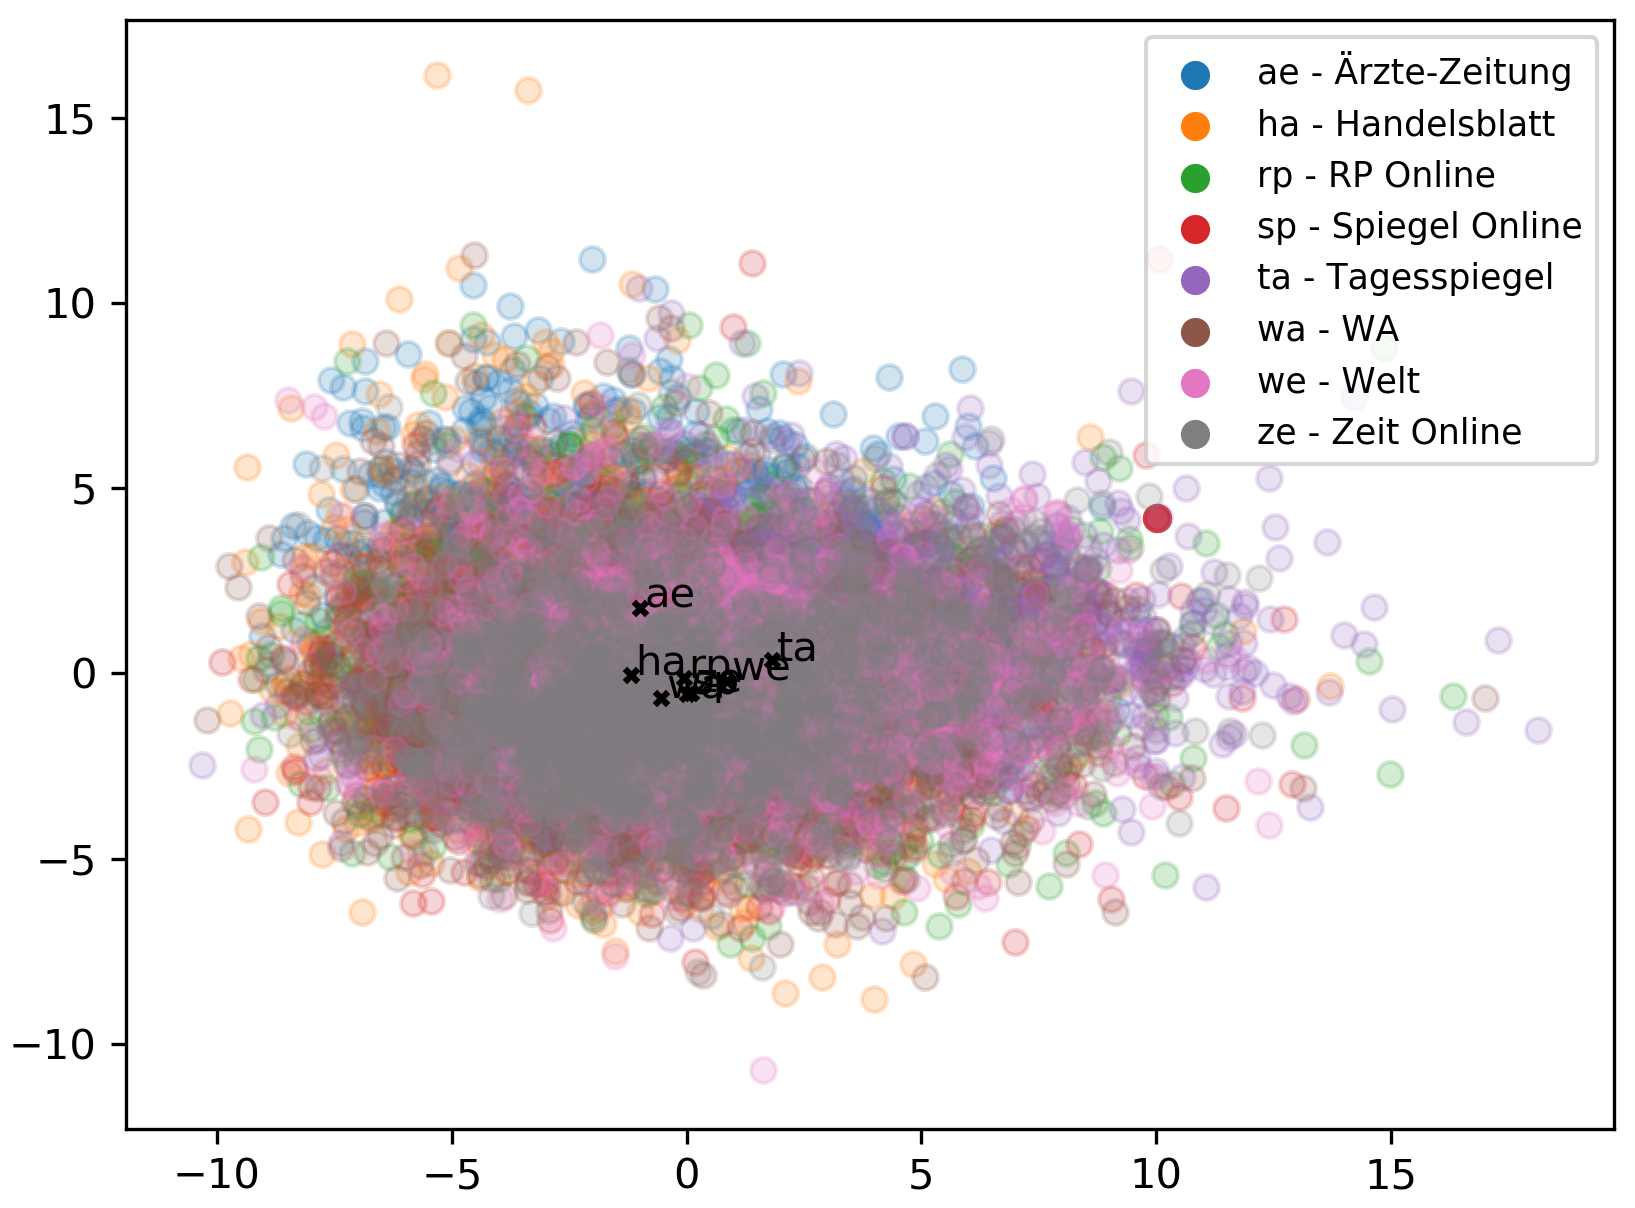
\includegraphics[width=\textwidth]{pca_all}
      \caption{PCA mit allen Features}
      \label{fig:pca_all}
  \end{subfigure}
  ~ %add desired spacing between images, e. g. ~, \quad, \qquad, \hfill etc. 
    %(or a blank line to force the subfigure onto a new line)
  \begin{subfigure}[b]{0.49\textwidth}
      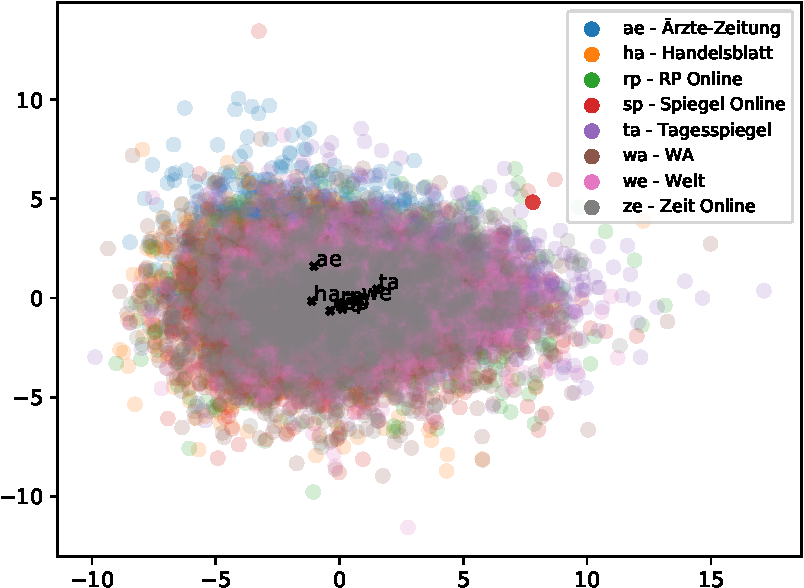
\includegraphics[width=\textwidth]{pca_best_80}
      \caption{PCA mit den besten 80 Features}
      \label{fig:pca_best_80}
  \end{subfigure}
  \caption{Hauptkomponentenanalyse (PCA) der Politik-Artikel}\label{fig:pca}
\end{figure}

Da das Clustering nach Hauptkomponentenanalyse keine guten Ergebnisse erzielen kann, wird zudem t-SNE eingesetzt, um Cluster der Artikel zu finden. Dieses Verfahren wird mit steigender Anzahl an Datenpunkten und vor allem höherer Dimensionalität sehr viel rechenintensiver. Daher wird die Anzahl der Artikel pro Zeitung auf etwa 1000 begrenzt und die Dimensionalität mithilfe von PCA auf 125 reduziert. Hierbei ist es notwendig, verschiedene Kombinationen aus der Anzahl an Iterationen \texttt{n\_iter}, der Lernrate \texttt{learning\_rate}, und des Parameters \texttt{perplexity}, zu testen, da diese Variablen großen Einfluss auf das Endergebnis besitzen. Für \texttt{n\_iter} werden 500, 1000 und 2000, für \texttt{learning\_rate} 10, 20, 40, 100 und 500 und für \texttt{perplexity} 10, 25, 50, 60, 75 und 100 als Werte verwendet. Aus allen 90 Kombinationen ergibt sich jedoch kein Diagramm, welches gute Cluster zeigt und Artikel der gleichen Zeitungen sind auch hier über den ganzen Raum verteilt. Abbildung \ref{img.tsne_temp} zeigt dabei das "'beste"' Ergebnis mit der Kombination \texttt{n\_iter = 2000}, \texttt{learning\_rate = 20} und \texttt{perplexity = 50}. Dabei ist zu beachten, dass die Distanzen der Punkte im Diagramm untereinander keine Bedeutung haben und das Verfahren nur Cluster findet und visuell darstellt. Folglich ist es nicht möglich, die Artikel oder Zeitungen anhand der in dieser Arbeit verwendeten Features zu gruppieren.

\bild{tsne_temp}{0.9\textwidth}{Clustering der Politik-Artikel mit dem t-SNE Verfahren}{Clustering der Politik-Artikel mit dem t-SNE Verfahren}
\todo{T-SNE Bild austauschen}

\chapter{Ergebnis}

\bibliographystyle{alphadin_martin}
\bibliography{bibliographie}

\chapter*{Erklärung}

Hiermit versichere ich, dass ich die vorliegende Arbeit selbstständig verfasst und keine anderen als die angegebenen Quellen und Hilfsmittel benutzt habe, dass alle Stellen der Arbeit, die wörtlich oder sinngemäß aus anderen Quellen übernommen wurden, als solche kenntlich gemacht und dass die Arbeit in gleicher oder ähnlicher Form noch keiner Prüfungsbehörde vorgelegt wurde.

\vspace{3cm}
Ort, Datum \hspace{5cm} Unterschrift\\

\end{document}